%% Presenter guide for the half-scope (mid-term) GTX-GPU presentation.
%% Build: pdflatex presenter_guide (twice). Needs tcolorbox, pgfplots, tikz.
\documentclass[11pt,a4paper]{article}
\usepackage[T1]{fontenc}
\usepackage{libertine}
\usepackage[libertine]{newtxmath}
\usepackage{inconsolata}
\usepackage[margin=2.3cm]{geometry}
\usepackage{microtype}
\usepackage{graphicx}
\usepackage{booktabs}
\usepackage{array}
\usepackage{enumitem}
\usepackage[most]{tcolorbox}
\usepackage{tikz}
\usetikzlibrary{arrows.meta,positioning,calc,shapes.misc,decorations.pathreplacing}
\usepackage{pgfplots}
\pgfplotsset{compat=1.18}
\usepackage[hidelinks]{hyperref}
\usepackage{titlesec}
\usepackage{float}

\definecolor{cGTX}{HTML}{1F5FA8}
\definecolor{cCONS}{HTML}{7AA6D6}
\definecolor{cORG}{HTML}{C8651B}
\definecolor{cHUB}{HTML}{D95F02}
\definecolor{cGRN}{HTML}{1B7F5E}
\definecolor{ink}{HTML}{152238}

\setlength{\parskip}{5pt}
\setlength{\parindent}{0pt}
\setlist{itemsep=2pt, topsep=3pt}
\titleformat{\section}{\Large\bfseries\color{ink}}{\thesection}{0.6em}{}
\titleformat{\subsection}{\large\bfseries\color{ink}}{\thesubsection}{0.6em}{}

\newcommand{\code}[1]{\texttt{#1}}

% Boxes used throughout
\newtcolorbox{oneline}{colback=cGTX!6, colframe=cGTX, fonttitle=\bfseries, title=If you remember only one sentence, left=6pt, right=6pt}
\newtcolorbox{sayit}{colback=cGRN!5, colframe=cGRN, fonttitle=\bfseries, title=What to say (script you can adapt), left=6pt, right=6pt, breakable}
\newtcolorbox{askme}{colback=cORG!6, colframe=cORG, fonttitle=\bfseries, title=Likely questions and simple answers, left=6pt, right=6pt, breakable}
\newtcolorbox{analogy}{colback=black!3, colframe=black!40, fonttitle=\bfseries, title=Everyday analogy, left=6pt, right=6pt}
\newtcolorbox{dont}{colback=red!4, colframe=red!55!black, fonttitle=\bfseries, title=Keep this for the final presentation, left=6pt, right=6pt}
\newtcolorbox{slides}{colback=black!2, colframe=ink, fonttitle=\bfseries, title=Suggested slides for this part, left=6pt, right=6pt, breakable}

\begin{document}

%% ------------------------------------------------------------------------------------------
\begin{center}
{\Huge\bfseries\color{ink} GTX-GPU: Presenter Guide}\\[6pt]
{\Large Mid-term presentation (Part 1 of 2)}\\[4pt]
{\normalsize Everything the three presenters need to understand and explain their part}
\end{center}
\vspace{4pt}

\section*{How to use this guide}
Every presenter should read \textbf{Sections 1 and 2} (the glossary and the big picture), then their own section in
depth, then the ``one sentence'' box of the other two parts, so that anyone can cover a teammate's question.

\begin{center}
\begin{tabular}{@{}llll@{}}
\toprule
Part & Presenter & Topic & Time \\
\midrule
Opening & Presenter 1 & What the project is, what today covers & 1 min \\
Part 1 & Presenter 1 & The problem and our idea (\S\ref{sec:p1}) & 4 min \\
Part 2 & Presenter 2 & How the design works (\S\ref{sec:p2}) & 4 min \\
Part 3 & Presenter 3 & Correctness and first benchmarks (\S\ref{sec:p3}) & 4 min \\
Close & Presenter 3 & What comes next, questions & 1 min \\
\bottomrule
\end{tabular}
\end{center}

\textbf{Scope of today.} This is the \emph{first half} of the project, told in the order the work was done:
(1)~understand the problem and the existing systems, (2)~design the GPU data structure and its update rules,
(3)~build it, check that it is correct, and measure the engine on its own. The comparison against other systems, the
stricter ``serializable'' correctness mode, and memory cleanup are the second half and are presented next time
(\S\ref{sec:later}).

\tableofcontents
\newpage

%% ==========================================================================================
\section{Glossary: words you will hear and say}
\label{sec:glossary}

\begin{center}
\renewcommand{\arraystretch}{1.25}
\begin{tabular}{@{}>{\raggedright\arraybackslash\bfseries}p{3.1cm}>{\raggedright\arraybackslash}p{12.2cm}@{}}
\toprule
Term & Meaning, in plain words \\
\midrule
Graph, vertex, edge & A network. Vertices are the things (users, accounts, road junctions); edges are the connections
  between them. An edge $(u,v)$ goes from $u$ to $v$. \\
Dynamic graph & A graph whose edges keep being inserted and deleted while people read it. \\
Hub vertex & A very popular vertex (a celebrity account) that a large share of all updates touch. Real graphs have
  these, and they are what make concurrency hard. \\
Transaction & A group of operations that must happen \emph{all together or not at all}, e.g.\ ``delete edge A and insert
  edge B''. Nobody may see only half of it. \\
Commit / abort & Commit = the transaction succeeded and its changes become visible. Abort = it clashed with another
  transaction, gives up, and retries. \\
Snapshot & A frozen, consistent view of the graph at one moment. A reader working on a snapshot is not disturbed by
  writers. \\
Snapshot isolation (SI) & The correctness guarantee we provide today: every transaction reads from a snapshot, and two
  transactions that change the same edge cannot both commit. \\
GPU thread, warp & A GPU runs thousands of threads. They are grouped in \emph{warps} of 32 that execute the same
  instruction at the same time, in lockstep. \\
Atomic operation & A tiny operation the hardware guarantees nobody can interrupt halfway, e.g.\ ``add 5 to this
  counter and tell me the old value'' (\code{fetch\_add}). \\
CAS & \emph{Compare-and-swap}: ``set this value to Y, but only if it is still X, which is what I saw a moment ago''. If
  someone changed it in between, the CAS fails and you look again. This is how threads cooperate without locks. \\
Lock & A ``reserved'' sign: only the holder may touch the data; everybody else waits. Locks are slow and risky on
  GPUs, which is why we avoid them. \\
Version / delta & One record of one change to one edge (``edge $u\to7$ inserted by transaction 12''). We never overwrite
  data; we add versions. \\
Epoch & A batch number. Transactions commit in numbered batches (epochs). \\
Frontier & The newest epoch whose transactions are \emph{all} finished. Readers take this number as their snapshot. \\
Throughput & How much work is done per second (transactions/s or edges/s). \\
Effective edges/s & Edge changes that actually changed the graph. Inserting an edge that already exists does nothing,
  so it is not counted. \\
Abort ratio & The fraction of attempts that had to give up and retry. Lower is better. \\
p50 / p99 latency & The time within which 50\% / 99\% of requests finish. p99 describes the slow tail. \\
GTX & A published CPU graph system (Zhou et al., SIGMOD 2025) whose design we adapt to the GPU. \\
GTX-GPU & Our system. \\
\bottomrule
\end{tabular}
\end{center}

%% ==========================================================================================
\section{The big picture in one page}
\label{sec:big}

\textbf{The problem.} Graphs such as social networks, payment networks and road networks change all the time. Many
changes only make sense in groups, and people keep reading the graph while it changes. GPUs are very good at updating
graphs quickly, but none of the existing GPU graph systems can apply a \emph{group} of changes safely while readers run.

\textbf{The idea.} A CPU system called GTX solves this problem on CPUs with one central trick: \emph{never overwrite
anything; store every change as a new version}. Readers look at the versions that existed when they started; writers
add new versions next to them, so neither blocks the other. We take this design to the GPU.

\textbf{What had to change.} A GPU is not a big CPU. Threads move in groups of 32, thousands of them hit the same popular
vertex at once, and nothing can be paused to reorganize memory. We redesigned three things: how storage grows (without
copying), how threads reserve space (one atomic per group, not per thread), and how conflicts are detected (exactly per
edge, not per group of edges). Commits happen in numbered batches, so readers never wait and never see half a
transaction.

\textbf{What we can show today.} The engine works, is checked read by read by an automatic checker (48 of 48 test
scenarios pass), processes 140--180 million edge inserts per second, is up to $1.8\times$ faster than a direct port of
GTX's rules, and lets readers finish 99\% of their work within 2.4~ms.

\begin{figure}[H]
\centering
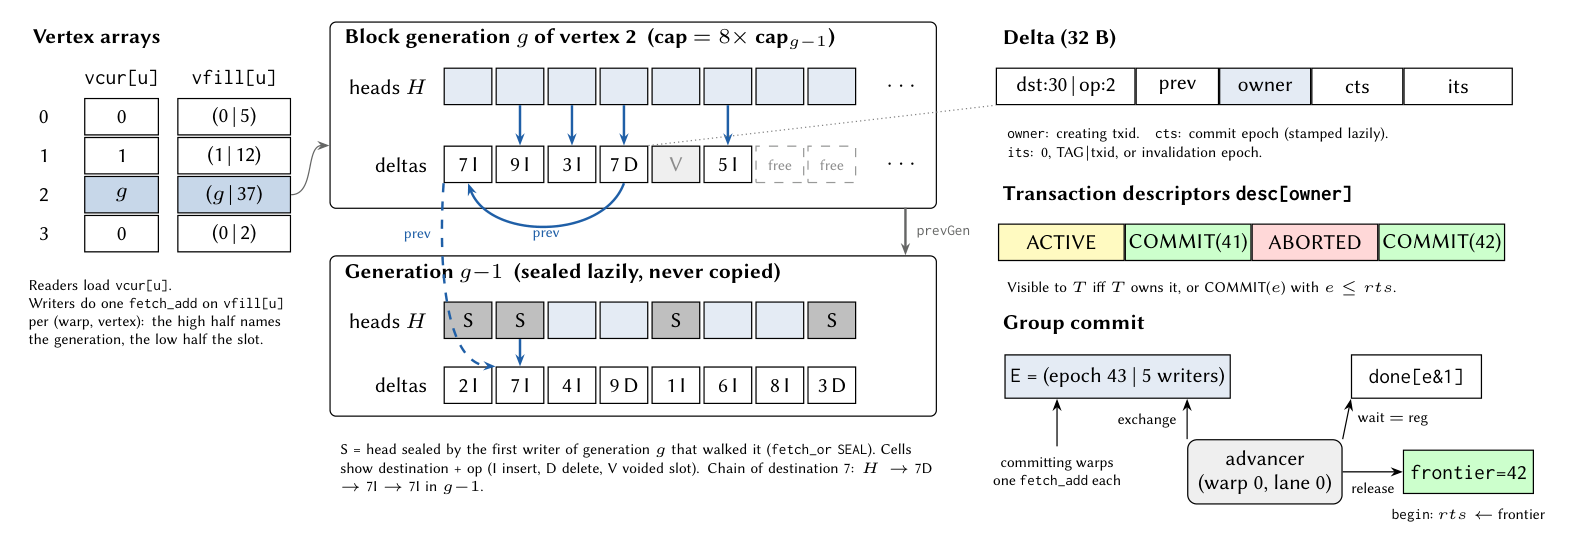
\includegraphics[width=\textwidth]{arch.png}
\caption{The whole system on one page (the same picture as Figure~1 of the technical report). Left: two small arrays
per vertex. Middle: the vertex's storage blocks, newest first, holding versions of its edges linked in chains. Right:
the layout of one version, the status table of transactions, and the batch-commit machinery. Presenter~2 explains the
left and middle; Presenter~3 explains the right.}
\label{fig:arch}
\end{figure}

\newpage
%% ==========================================================================================
\section{Presenter 1: The problem and our idea}
\label{sec:p1}

\begin{oneline}
GPUs can update graphs very fast, but not safely in groups. We are bringing a proven CPU design, GTX, to the GPU to
fix that.
\end{oneline}

\subsection{Why graphs need transactions}
Many real updates are not one edge but several edges that belong together:
\begin{itemize}
\item \textbf{Moving a connection.} A user switches from following account A to following account B: delete
  $(\text{user},A)$, insert $(\text{user},B)$.
\item \textbf{Undirected edges.} A friendship is stored in both directions: insert $(u,v)$ \emph{and} $(v,u)$.
\item \textbf{Edge plus a counter.} Add an edge and increase the vertex's degree (its number of edges).
\end{itemize}

If other threads read the graph while such a group is half done, they see a state that never really existed.
Figure~\ref{fig:torn} shows it: a reader that looks between the two steps sees the user following \emph{nobody}. That
reader might be a recommendation job or a fraud check, and it would compute a wrong answer.

\begin{figure}[H]
\centering
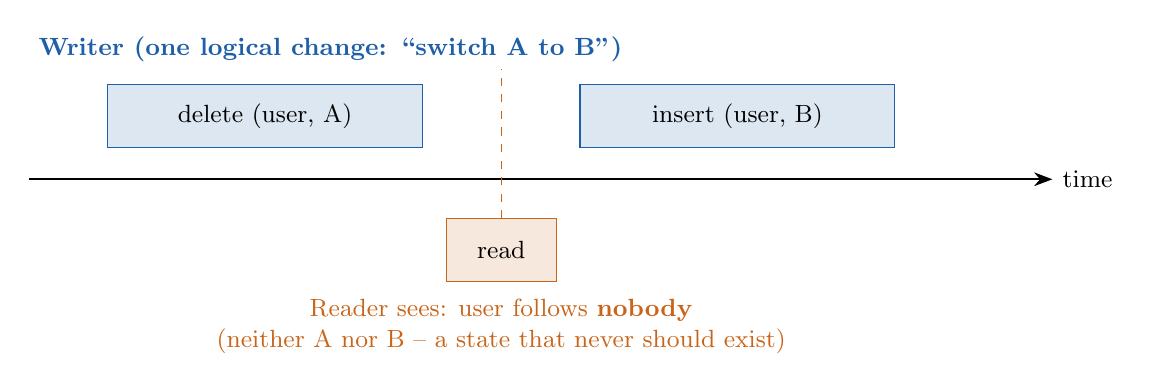
\begin{tikzpicture}[font=\small, >=Stealth]
\draw[->, thick] (0,0) -- (13,0) node[right] {time};
\draw[fill=cGTX!15, draw=cGTX] (1,0.4) rectangle (5,1.2) node[midway] {delete (user, A)};
\draw[fill=cGTX!15, draw=cGTX] (7,0.4) rectangle (11,1.2) node[midway] {insert (user, B)};
\node[cGTX, anchor=west] at (0,1.65) {\textbf{Writer (one logical change: ``switch A to B'')}};
\draw[fill=cORG!15, draw=cORG] (5.3,-1.3) rectangle (6.7,-0.5) node[midway] {read};
\node[cORG, align=center, anchor=north] at (6,-1.4) {Reader sees: user follows \textbf{nobody}\\ (neither A nor B -- a state that never should exist)};
\draw[dashed, cORG] (6,-0.5) -- (6,1.4);
\end{tikzpicture}
\caption{A ``torn read''. Without transactions, a reader can observe half of a group of changes.}
\label{fig:torn}
\end{figure}

So we need two guarantees:
\begin{enumerate}
\item \textbf{All-or-nothing groups} (transactions): the two changes happen together or not at all.
\item \textbf{Consistent reading during updates} (snapshots): a reader sees the graph as it was at one moment, never
  half of a transaction.
\end{enumerate}

\subsection{Why GPUs, and what exists today}
GPUs have thousands of threads and far more memory bandwidth than a CPU, and much graph analytics already runs on them.
Several GPU structures for dynamic graphs exist, and they are fast: SlabGraph, for example, reports 500--640 million
edge insertions per second. But they all work \emph{batch at a time}: you hand them a big batch of updates, they apply
it, and during that time nobody may read. None offers groups of changes that are all-or-nothing, or safe reading
during updates.

\begin{center}
\renewcommand{\arraystretch}{1.15}
\begin{tabular}{@{}>{\raggedright\arraybackslash}p{3.8cm}>{\raggedright\arraybackslash}p{3.6cm}>{\raggedright\arraybackslash}p{2.5cm}>{\raggedright\arraybackslash}p{3.8cm}@{}}
\toprule
System & How it stores edges & Transactions? & Safe reads during updates? \\
\midrule
GPMA, GPMA+, LPMA & sorted arrays & no (batches) & no \\
Hornet, faimGraph & per-vertex arrays / pages & no & no \\
SlabGraph, Meerkat & per-vertex hash tables & no & no \\
GPU transactional memory (GPU-STM, PR-STM, CSMV) & any memory, not graph-aware & yes & yes, but slow on graphs \\
GTX (CPU only) & versioned edge records & yes & yes \\
\textbf{GTX-GPU (ours)} & versioned edge records & \textbf{yes} & \textbf{yes} \\
\bottomrule
\end{tabular}
\end{center}

\textbf{Why not just use GPU transactional memory?} It treats memory as anonymous words and knows nothing about edges.
Every insert into a popular vertex also updates that vertex's edge counter, so thousands of unrelated transactions
collide on that single counter and keep aborting each other. You only need to say this qualitatively today; the
measurements belong to the final presentation.

\subsection{The GTX idea: never overwrite, add versions}
GTX (a SIGMOD 2025 CPU system) keeps, for every vertex, a list of \emph{versions}. Each version records one change to one
edge and \emph{when} it happened. Its four ideas, which we keep:
\begin{enumerate}
\item \textbf{Versions instead of overwrites.} Readers look at old versions while writers add new ones, so readers never
  wait for writers.
\item \textbf{Per-edge chains.} The versions of one edge are linked together, so a writer can quickly check whether
  someone else is changing the same edge.
\item \textbf{Status lookup on demand.} A version knows which transaction wrote it; a reader checks that transaction's
  status (still running, committed, aborted) only when it meets the version.
\item \textbf{Batch commits.} Transactions commit in numbered batches; a reader's snapshot is simply ``everything up to
  batch $N$''.
\end{enumerate}
GTX reports up to $11\times$ higher throughput than earlier CPU graph systems (LiveGraph, Teseo, Sortledton).

\begin{analogy}
A shared notebook where nobody ever erases. To change a phone number you write a new line with a timestamp. Someone
reading ``as of 10:00'' simply ignores lines written after 10:00, so they never have to wait for the writer, and they
never see a half-written entry.
\end{analogy}

\subsection{Why a GPU needs changes}
\begin{itemize}
\item \textbf{Lockstep groups of 32.} A warp's 32 threads execute together and often target the same hub vertex. If each
  thread performs its own atomic operation on that vertex, they queue up one after another. A thread waiting for a
  lock inside a warp can even block the thread that holds it (deadlock).
\item \textbf{No ``stop the world''.} GTX copies a vertex's storage into a bigger block when it is full. On a GPU,
  thousands of threads may be writing into that block at that instant, so it cannot be copied safely.
\item \textbf{Bugs are silent.} GPU memory ordering is weak: if one ``publish'' step is missing, nothing crashes; a rare
  reader just sees wrong data. So we need a strong way to prove the system is correct (Presenter~3).
\end{itemize}

\textbf{Our goal:} keep GTX's architecture, and redesign exactly the parts the GPU breaks.

\begin{sayit}
``Graphs like social or payment networks change constantly, and many changes come in groups, like unfollowing one
account and following another. If someone reads in the middle, they see a state that should never exist
(Figure~\ref{fig:torn}). So we need two things: all-or-nothing groups, and readers that always see a consistent
picture.

GPUs are the fastest hardware for graph updates today, and there are several GPU graph systems, but they all apply
updates in big batches with nobody reading. None of them supports safe groups of changes. General GPU transactional
memory does, but it doesn't understand graphs, so on popular vertices everything collides.

On CPUs, a system called GTX solved this with one idea: never overwrite, always add a new version. Readers look at
older versions while writers add new ones. We are bringing GTX to the GPU. That's not a simple port: GPU threads run
in lockstep groups of 32, thousands of them hit the same popular vertex, and nothing can be paused to reorganize
memory. [Presenter 2] will show how we redesigned it.''
\end{sayit}

\begin{askme}
\textbf{Why not do this on a CPU?} GPUs offer far more parallelism and memory bandwidth, and graph analytics already
runs on GPUs; moving the graph back and forth between CPU and GPU is expensive.

\textbf{Is GTX your system?} No. GTX is a published CPU system (Zhou et al., SIGMOD 2025). Ours is GTX-GPU: the GPU
adaptation and its new mechanisms.

\textbf{What guarantee do you give?} Snapshot isolation today (defined in the glossary). A stricter mode
(serializability) is part of the next stage.
\end{askme}

\begin{slides}
\begin{enumerate}[leftmargin=*]
\item Title and team; one-line pitch; ``today = first half: problem, design, first results''.
\item ``Graph updates come in groups'': the follow/unfollow example and Figure~\ref{fig:torn}.
\item ``No GPU system offers both'': the table above.
\item ``GTX: never overwrite, add versions'': four ideas and the notebook analogy.
\item ``Why the GPU needs changes'': three bullets, then the goal sentence.
\end{enumerate}
\end{slides}

\newpage
%% ==========================================================================================
\section{Presenter 2: How the design works}
\label{sec:p2}

\begin{oneline}
We keep every version of every edge, we grow storage without copying it, and threads coordinate with single atomic
operations and ``check-then-swap'' instead of locks.
\end{oneline}

Use Figure~\ref{fig:arch} as your anchor slide. Point at three things only: the versions (middle), the storage blocks
(middle, top and bottom), and the small per-vertex arrays (left).

\subsection{Idea 1: versions, not overwrites}
For every vertex we keep a list of small records (32 bytes each), one per change. Each record stores:
\begin{itemize}
\item \textbf{which edge and what happened}: the destination vertex and the operation (\emph{insert} or \emph{delete});
\item \textbf{who wrote it}: the id of the transaction that created it;
\item \textbf{when it became official}: the commit batch number (filled in after commit);
\item \textbf{a link to the previous version of the same edge}, which forms a chain per edge.
\end{itemize}

The current state of an edge, for a given reader, is simply the \emph{newest version that reader is allowed to see}.
A delete is not an erase; it is a new record saying ``deleted''. Figure~\ref{fig:chain} shows the chain for one edge.

\begin{figure}[H]
\centering
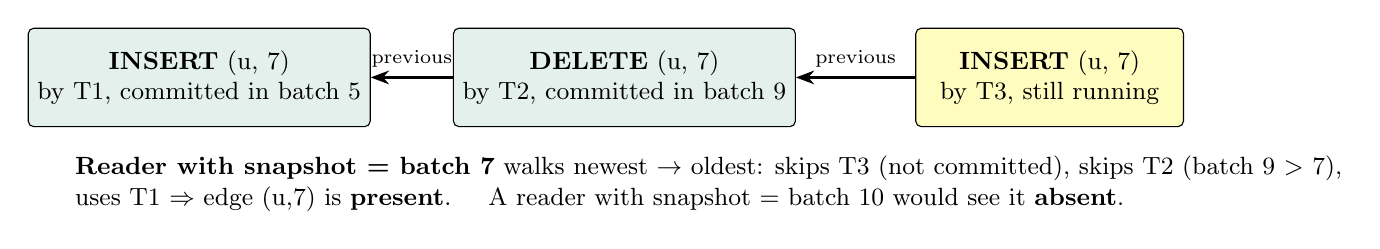
\begin{tikzpicture}[font=\small, >=Stealth,
  ver/.style={draw, rounded corners=2pt, minimum width=3.4cm, minimum height=1.25cm, align=center}]
\node[ver, fill=cGRN!12] (v1) at (0,0) {\textbf{INSERT} (u, 7)\\ by T1, committed in batch 5};
\node[ver, fill=cGRN!12] (v2) at (5.4,0) {\textbf{DELETE} (u, 7)\\ by T2, committed in batch 9};
\node[ver, fill=yellow!25] (v3) at (10.8,0) {\textbf{INSERT} (u, 7)\\ by T3, still running};
\draw[->, thick] (v3) -- node[above, font=\scriptsize] {previous} (v2);
\draw[->, thick] (v2) -- node[above, font=\scriptsize] {previous} (v1);
\node[anchor=west, align=left] at (-1.7,-1.35) {\textbf{Reader with snapshot = batch 7} walks newest $\rightarrow$ oldest:
  skips T3 (not committed), skips T2 (batch 9 $>$ 7),\\ uses T1 $\Rightarrow$ edge (u,7) is \textbf{present}.
  \quad A reader with snapshot = batch 10 would see it \textbf{absent}.};
\end{tikzpicture}
\caption{Three versions of one edge. Different readers see different, but always consistent, states.}
\label{fig:chain}
\end{figure}

Two useful consequences:
\begin{itemize}
\item \textbf{Readers never wait.} They just skip versions that are too new.
\item \textbf{Aborting is free.} If a transaction fails, its versions stay in memory but are ignored forever, because
  its status says ``aborted''. Nothing needs to be undone.
\end{itemize}

\subsection{Idea 2: growing storage without copying}
Each vertex's versions live in a storage block. When the block is full, GTX on the CPU copies everything into a bigger
block. On the GPU, thousands of threads may be writing into that block at that exact moment, so we never copy:
\begin{enumerate}
\item The thread that asks for the first slot \emph{beyond} the end is, by construction, the only one; it becomes the
  ``grower''.
\item It creates a new block \textbf{8$\times$ larger} and links it \emph{in front of} the old one (Figure~\ref{fig:grow}).
\item It publishes the new block; other threads that were waiting simply retry and land in the new block.
\item The old block stays where it is and is still read. The first writer that later walks an edge's chain into the
  old block marks (``seals'') that chain there, so from then on that edge's new versions only go into the newest block.
  This keeps all versions of an edge in one clean order.
\end{enumerate}

\begin{figure}[H]
\centering
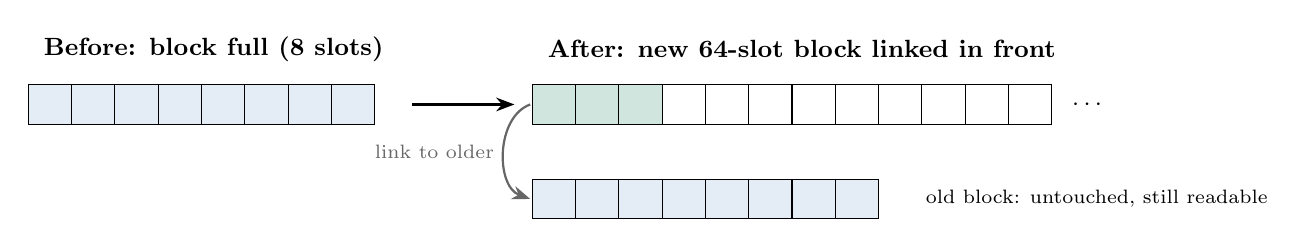
\begin{tikzpicture}[font=\small, >=Stealth, s/.style={draw, minimum width=0.55cm, minimum height=0.5cm}]
\node[anchor=west] at (-0.2,1.3) {\textbf{Before: block full (8 slots)}};
\foreach \i in {0,...,7} \node[s, fill=cGTX!12] at (\i*0.55,0.6) {};
\node[anchor=west] at (6.2,1.3) {\textbf{After: new 64-slot block linked in front}};
\foreach \i in {0,...,11} \node[s, fill=white] (n\i) at (6.4+\i*0.55,0.6) {};
\foreach \i in {0,1,2} \node[s, fill=cGRN!20] at (6.4+\i*0.55,0.6) {};
\node at (13.2,0.6) {$\cdots$};
\foreach \i in {0,...,7} \node[s, fill=cGTX!12] (o\i) at (6.4+\i*0.55,-0.6) {};
\draw[->, thick, black!60] (6.1,0.6) to[out=200,in=160] node[left, font=\scriptsize] {link to older} (6.1,-0.6);
\node[anchor=west, font=\scriptsize] at (11.0,-0.6) {old block: untouched, still readable};
\draw[->, thick] (4.6,0.6) -- (5.9,0.6);
\end{tikzpicture}
\caption{Growth by generations. Nothing is copied; new versions go into the new block (green).}
\label{fig:grow}
\end{figure}

\begin{analogy}
When a notebook is full you do not rewrite it into a bigger notebook while ten people are writing in it. You put a
new, thicker notebook on top of the old one and write there; the old notebook is still on the shelf if you need to
look something up.
\end{analogy}

\subsection{Idea 3: coordinating without locks}
\textbf{Getting a slot: one atomic per group, not per thread.}
Each vertex has a counter ``how many slots are used'' (\code{vfill} in Figure~\ref{fig:arch}). Normally every thread
that wants to write would increase it with its own atomic operation, and on a hub vertex 32 threads would queue on the
same counter. Instead, the threads of a warp that target the same vertex first form a group (one GPU instruction,
\code{\_\_match\_any\_sync}); the group leader increases the counter \emph{once} by the group size, and every thread takes
``start + its position in the group'' (Figure~\ref{fig:resv}). A detail worth one sentence: the same 64-bit word stores
both \emph{which block} is current and \emph{how many slots} are used, so one atomic answers both questions at once and a
thread can never end up with a slot in the wrong block.

\begin{figure}[H]
\centering
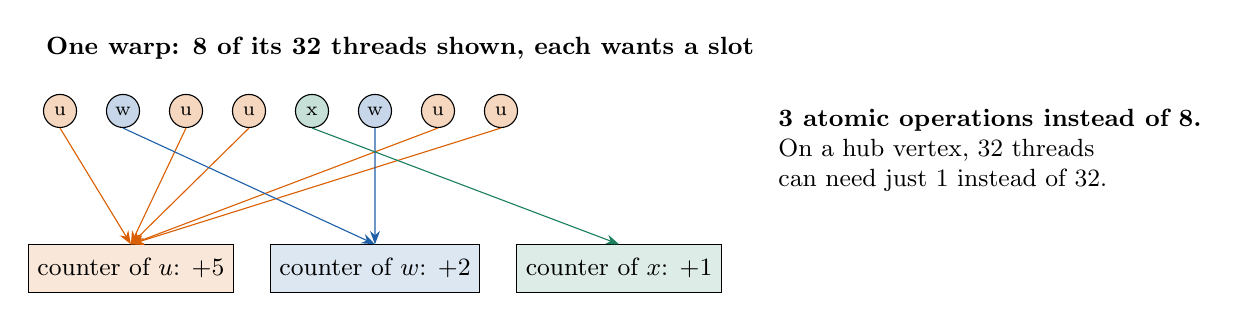
\begin{tikzpicture}[font=\small, >=Stealth, l/.style={draw, circle, minimum size=0.42cm, inner sep=0pt, font=\scriptsize}]
\node[anchor=west] at (-0.3,1.0) {\textbf{One warp: 8 of its 32 threads shown, each wants a slot}};
\foreach \i/\c/\v in {0/cHUB/u,1/cGTX/w,2/cHUB/u,3/cHUB/u,4/cGRN/x,5/cGTX/w,6/cHUB/u,7/cHUB/u}
  \node[l, fill=\c!25] (t\i) at (\i*0.8,0.2) {\v};
\node[draw, fill=cHUB!15, minimum height=0.6cm] (cu) at (0.9,-1.8) {counter of $u$: +5};
\node[draw, fill=cGTX!15, minimum height=0.6cm] (cw) at (4.0,-1.8) {counter of $w$: +2};
\node[draw, fill=cGRN!15, minimum height=0.6cm] (cx) at (7.1,-1.8) {counter of $x$: +1};
\foreach \i in {0,2,3,6,7} \draw[->, cHUB] (t\i.south) -- (cu.north);
\foreach \i in {1,5} \draw[->, cGTX] (t\i.south) -- (cw.north);
\draw[->, cGRN] (t4.south) -- (cx.north);
\node[anchor=west, align=left, font=\small] at (9.0,-0.3) {\textbf{3 atomic operations instead of 8.}\\ On a hub vertex, 32 threads\\ can need just 1 instead of 32.};
\end{tikzpicture}
\caption{Warp-cooperative reservation. Threads that want space in the same vertex share one atomic operation.}
\label{fig:resv}
\end{figure}

\textbf{Linking a new version: check, then swap.}
To insert or delete edge $(u,v)$, a thread:
\begin{enumerate}
\item reads the current start (``head'') of the chain for $v$;
\item walks the versions of $v$ in that chain: if another transaction that is still running has a version there, or a
  version was committed after its own snapshot, the two would conflict, so it \textbf{aborts} and retries later;
\item otherwise writes its version and links it with a \textbf{CAS on the same head it checked}: ``make my version the
  head, but only if the head is still what I checked'';
\item if the CAS fails (someone linked something in between), it checks \emph{only the new part}; if that part touches
  the same edge, it aborts, otherwise it simply tries again.
\end{enumerate}
Figure~\ref{fig:cas} shows two threads racing for the same edge: exactly one wins, the other notices and aborts. No
lock is ever held, so no thread waits for another.

\begin{figure}[H]
\centering
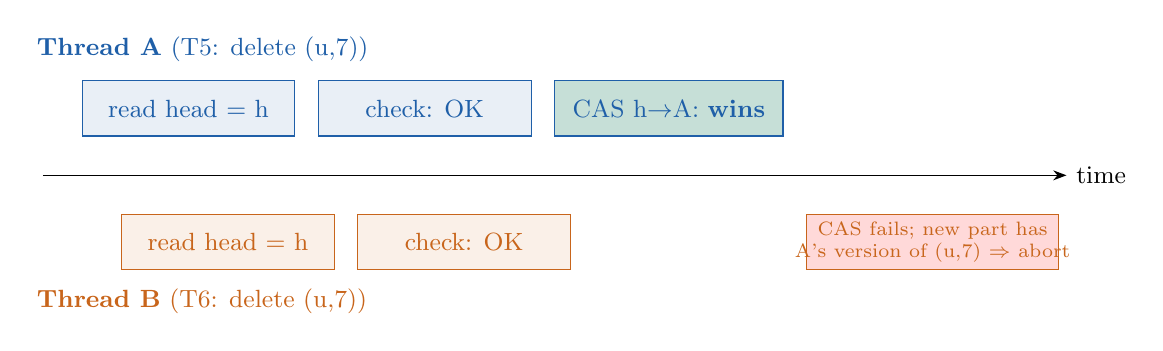
\begin{tikzpicture}[font=\small, >=Stealth]
\draw[->] (0,0) -- (13,0) node[right] {time};
\node[anchor=west, cGTX] at (-0.2,1.6) {\textbf{Thread A} (T5: delete (u,7))};
\node[anchor=west, cORG] at (-0.2,-1.6) {\textbf{Thread B} (T6: delete (u,7))};
\draw[cGTX, fill=cGTX!10] (0.5,0.5) rectangle (3.2,1.2) node[midway] {read head = h};
\draw[cGTX, fill=cGTX!10] (3.5,0.5) rectangle (6.2,1.2) node[midway] {check: OK};
\draw[cGTX, fill=cGRN!25] (6.5,0.5) rectangle (9.4,1.2) node[midway] {CAS h$\to$A: \textbf{wins}};
\draw[cORG, fill=cORG!10] (1.0,-1.2) rectangle (3.7,-0.5) node[midway] {read head = h};
\draw[cORG, fill=cORG!10] (4.0,-1.2) rectangle (6.7,-0.5) node[midway] {check: OK};
\draw[cORG, fill=red!15] (9.7,-1.2) rectangle (12.9,-0.5) node[midway, align=center, font=\scriptsize] {CAS fails; new part has\\ A's version of (u,7) $\Rightarrow$ abort};
\end{tikzpicture}
\caption{Check-then-swap. Both threads checked the same head; only the first CAS succeeds. The loser re-checks only
what changed, sees a conflicting version of the same edge, and aborts.}
\label{fig:cas}
\end{figure}

\textbf{How this differs from GTX.} GTX's rule is coarser: several edges share one chain, and GTX aborts if the newest
version on the chain is not visible, \emph{whichever edge it belongs to}. Two transactions touching \emph{different}
edges that happen to share a chain then abort each other for no reason. Our rule only looks at versions of the
\emph{same} edge. Presenter~3 shows what this is worth in numbers (Figure~\ref{fig:aborts}).

\begin{sayit}
``Here is the whole system on one page [Figure~\ref{fig:arch}]. Three ideas.

First, we never overwrite. Every change to an edge is a small new record: which edge, insert or delete, which
transaction wrote it, and when it committed. The versions of one edge form a chain. A reader walks the chain from
newest to oldest and takes the first version it is allowed to see [Figure~\ref{fig:chain}]. So readers never wait,
and if a transaction fails, there is nothing to undo; its records are simply ignored.

Second, storage grows without copying. When a vertex's block is full, exactly one thread creates a block eight times
bigger and links it in front. The old block stays readable. On a GPU that matters, because thousands of threads may be
writing into that block at that moment [Figure~\ref{fig:grow}].

Third, no locks. Threads in a warp that want space in the same vertex share one atomic operation instead of each doing
their own [Figure~\ref{fig:resv}]. To add a version, a thread checks the chain of that exact edge and then links its
version with compare-and-swap, `only if nothing changed since I looked'. If two threads race for the same edge, exactly
one wins and the other aborts and retries [Figure~\ref{fig:cas}]. GTX checks conflicts more coarsely, which causes
unnecessary aborts; [Presenter 3] will show the difference, and how we know all this is correct.''
\end{sayit}

\begin{askme}
\textbf{Doesn't keeping every version use a lot of memory?} Yes. Cleaning up versions nobody can see any more is
planned for the next stage.

\textbf{Why 8$\times$ bigger blocks?} Growing by a large factor means growth happens rarely, so the (rare) waiting for
the one growing thread is negligible.

\textbf{What if two threads want the same slot?} They can't: one atomic operation hands out distinct slot numbers.

\textbf{Is compare-and-swap a lock?} No. Nobody holds anything; a failed CAS just means ``look again''. Someone else's
CAS succeeded, so the system as a whole always makes progress.
\end{askme}

\begin{slides}
\begin{enumerate}[leftmargin=*]
\item ``The whole system on one page'': Figure~\ref{fig:arch}.
\item ``Every change is a new version'': Figure~\ref{fig:chain}.
\item ``Storage grows without copying'': Figure~\ref{fig:grow} and the notebook analogy.
\item ``One atomic per group'': Figure~\ref{fig:resv}.
\item ``Check, then swap'': Figure~\ref{fig:cas}, plus the one-line contrast with GTX.
\end{enumerate}
\end{slides}

\newpage
%% ==========================================================================================
\section{Presenter 3: Correctness and first benchmarks}
\label{sec:p3}

\begin{oneline}
Readers see consistent batches and never wait; an automatic checker verifies every single read and everything passes;
and the engine already processes over 100 million edge updates per second, up to 1.8$\times$ faster than GTX's
original rules.
\end{oneline}

\subsection{How readers stay consistent: batches (epochs)}
Transactions commit in numbered batches called \emph{epochs}. The mechanism has three players (right-hand side of
Figure~\ref{fig:arch}):
\begin{itemize}
\item \textbf{Committing transactions} join the currently open batch. A whole warp joins with \emph{one} atomic
  operation on a single counter that holds both ``current batch number'' and ``how many writers joined''. The
  transaction then marks itself ``committed in batch $e$'' and reports ``done''.
\item \textbf{One special thread, the advancer}, closes the open batch (opening the next one), waits until every writer
  that joined the closed batch has reported done, and only then announces: ``batch $e$ is complete'', by updating a
  single number called the \textbf{frontier}.
\item \textbf{A reader} starts by reading the frontier; that number is its snapshot. It then sees exactly the versions
  of batches up to the frontier (Figure~\ref{fig:chain}).
\end{itemize}

\begin{figure}[H]
\centering
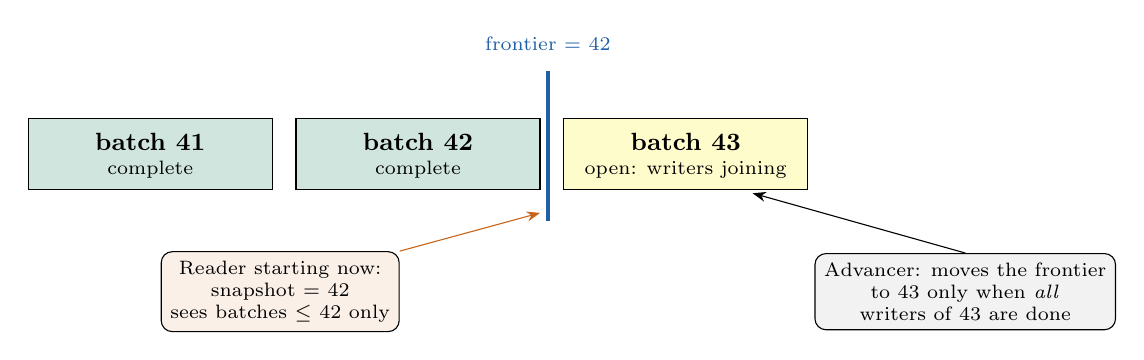
\begin{tikzpicture}[font=\small, >=Stealth]
\foreach \e/\x/\c/\t in {41/0/cGRN/complete, 42/3.4/cGRN/complete, 43/6.8/yellow/open: writers joining} {
  \draw[fill=\c!20] (\x,0) rectangle (\x+3.1,0.9);
  \node at (\x+1.55,0.6) {\textbf{batch \e}};
  \node[font=\scriptsize] at (\x+1.55,0.25) {\t};
}
\draw[very thick, cGTX] (6.6,-0.4) -- (6.6,1.5);
\node[cGTX, align=center, font=\scriptsize] at (6.6,1.85) {frontier = 42};
\node[draw, rounded corners, fill=cORG!10, align=center, font=\scriptsize] (r) at (3.2,-1.3) {Reader starting now:\\ snapshot = 42\\ sees batches $\le$ 42 only};
\draw[->, cORG] (r.north east) -- (6.5,-0.3);
\node[draw, rounded corners, fill=black!5, align=center, font=\scriptsize] (a) at (11.9,-1.3) {Advancer: moves the frontier\\ to 43 only when \emph{all}\\ writers of 43 are done};
\draw[->] (a.north) -- (9.2,-0.05);
\end{tikzpicture}
\caption{Batch commit. Because the frontier only moves past a batch when every transaction in it is finished, a reader
can never see half a transaction, and it never has to wait.}
\label{fig:epochs}
\end{figure}

\textbf{Why this matters:} a transaction's versions all carry the same batch number, and readers only see complete
batches. So a reader sees either \emph{all} of a transaction or \emph{none} of it, with no waiting and no locks.

\textbf{A story worth telling (it shows real engineering).} Our first version of ``join the batch'' read the batch number,
registered, then read it again to make sure it had not changed, and retried if it had. The advancer changes the batch
number about once per microsecond, so under load a committing thread kept retrying and a run that should take 1~ms
sometimes took 1.5--20 seconds (a \emph{livelock}). Packing the batch number and the writer count into one word, so that
joining is a single atomic operation that always succeeds, fixed it: 180 of 180 repeated runs then finished in
0.15--1.0~ms.

\subsection{How we know it is correct: the history checker}
GPU concurrency bugs rarely crash; they produce a \emph{wrong read} once in a million operations. The usual test in GPU
prototypes (``does the final graph equal the list of logged changes?'') cannot see such bugs. Example: two
transactions both delete the same edge and both report success. The final graph looks fine (the edge is gone), but
one of them should have aborted.

So every run records, for every transaction, its snapshot number, its commit batch, and the result of \emph{every}
operation. A checker on the CPU then replays the history and verifies:
\begin{enumerate}
\item \textbf{Every read is right:} each lookup and scan returned exactly what the graph looked like at that
  transaction's snapshot (plus its own earlier changes).
\item \textbf{The right version was read:} a lookup names the exact version it saw, never one from an aborted or
  unfinished transaction.
\item \textbf{No lost updates:} two transactions that changed the same edge never overlap in time.
\item \textbf{The final graph is right.}
\item A fifth check (no ordering cycles) is used for the stricter mode planned for the next stage.
\end{enumerate}

\textbf{Results.}
\begin{itemize}
\item \textbf{48 of 48} adversarial test histories pass: six nasty workloads (tiny graphs with heavy collisions, a hub
  vertex taking 50\% of operations, 8 edges everyone fights over, delete/re-insert churn, large transactions, many readers)
  $\times$ 8 configurations.
\item \textbf{The checker catches bugs:} we deliberately broke the system in three ways (no conflict check, readers ignore
  their snapshot, readers see unfinished data). The checker caught all three, with thousands of violations each. Two of
  the three \emph{pass} the simple final-graph test, which is exactly why we built the checker.
\item Running out of memory is handled safely: the transactions that did commit are still consistent.
\end{itemize}

\subsection{First benchmarks}
\textbf{Setup (say this once).} Laptop GPU: NVIDIA RTX 4060 (8~GB), CUDA 12.8. Graph with $2^{20}\approx$ 1 million
vertices and 4 million starting edges; each run processes about 1 million operations. Each number is the median of 5
runs after a warm-up run.

\textbf{Workload names.} \emph{Uniform}: edges between random vertices, so few collisions. \emph{50\% hub}: half of all
operations touch one single vertex, a worst case for collisions. \emph{Zipf} and \emph{R-MAT}: realistic ``few very
popular, many unpopular'' graphs. $K$ = the number of edge operations per transaction. \emph{GTX rules} = our engine run
with GTX's original, coarser conflict rule and per-thread reservation, i.e.\ a direct port of GTX.

\subsubsection*{Benchmark 1: speed as transactions grow}
\begin{figure}[H]
\centering
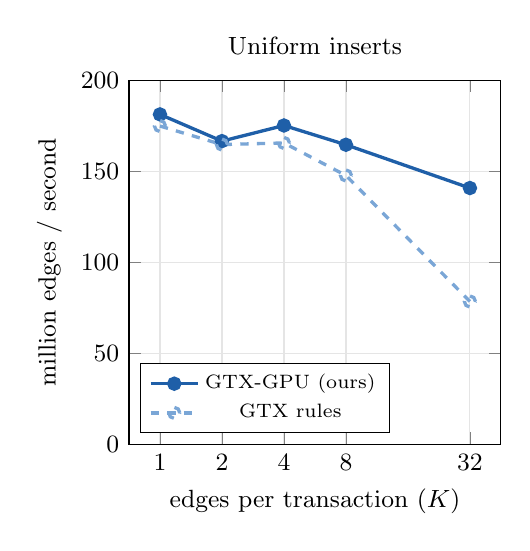
\begin{tikzpicture}
\begin{axis}[width=0.52\textwidth, height=6.2cm,
  xmode=log, log basis x=2, xtick={1,2,4,8,32}, xticklabels={1,2,4,8,32},
  ymin=0, ymax=200, grid=major, grid style={black!10},
  xlabel={edges per transaction ($K$)}, ylabel={million edges / second},
  title={\small Uniform inserts}, tick label style={font=\small}, label style={font=\small},
  legend style={font=\scriptsize, at={(0.03,0.03)}, anchor=south west}]
\addplot[cGTX, very thick, mark=*] coordinates {(1,181.4)(2,166.7)(4,175.3)(8,164.7)(32,140.9)};
\addlegendentry{GTX-GPU (ours)}
\addplot[cCONS, very thick, dashed, mark=o] coordinates {(1,175.0)(2,164.8)(4,165.7)(8,147.8)(32,78.5)};
\addlegendentry{GTX rules}
\end{axis}
\end{tikzpicture}\hfill
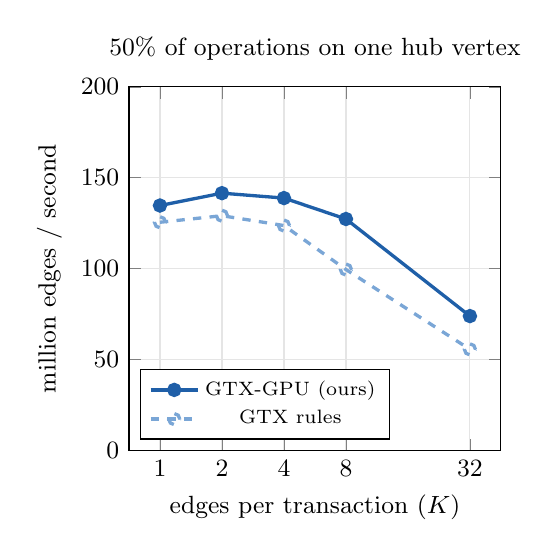
\begin{tikzpicture}
\begin{axis}[width=0.52\textwidth, height=6.2cm,
  xmode=log, log basis x=2, xtick={1,2,4,8,32}, xticklabels={1,2,4,8,32},
  ymin=0, ymax=200, grid=major, grid style={black!10},
  xlabel={edges per transaction ($K$)}, ylabel={million edges / second},
  title={\small 50\% of operations on one hub vertex}, tick label style={font=\small}, label style={font=\small},
  legend style={font=\scriptsize, at={(0.03,0.03)}, anchor=south west}]
\addplot[cGTX, very thick, mark=*] coordinates {(1,134.7)(2,141.5)(4,138.8)(8,127.3)(32,73.9)};
\addlegendentry{GTX-GPU (ours)}
\addplot[cCONS, very thick, dashed, mark=o] coordinates {(1,125.5)(2,129.1)(4,123.7)(8,99.5)(32,55.6)};
\addlegendentry{GTX rules}
\end{axis}
\end{tikzpicture}
\caption{Effective edge insertions per second. Our engine stays at 140--180 million/s on uniform graphs for every
transaction size, and above 120 million/s up to $K=8$ even when half of all operations hit one vertex.}
\label{fig:ksweep}
\end{figure}

\begin{center}
\begin{tabular}{@{}lrrrrr@{}}
\toprule
Million effective edges/s, by $K$ & 1 & 2 & 4 & 8 & 32 \\
\midrule
Uniform, GTX-GPU & 181.4 & 166.7 & 175.3 & 164.7 & 140.9 \\
Uniform, GTX rules & 175.0 & 164.8 & 165.7 & 147.8 & 78.5 \\
50\% hub, GTX-GPU & 134.7 & 141.5 & 138.8 & 127.3 & 73.9 \\
50\% hub, GTX rules & 125.5 & 129.1 & 123.7 & 99.5 & 55.6 \\
\bottomrule
\end{tabular}
\end{center}

\textbf{How to read it:} flat lines are good; they mean bigger transactions do not make the system slower per edge.
Ours stays flat; GTX's rules drop sharply at $K=32$. On the hub workload even ours drops at $K=32$, because 32-edge
transactions that all touch the same vertex genuinely collide (these are real conflicts, not false ones).

\subsubsection*{Benchmark 2: our conflict rule removes unnecessary aborts}
\begin{figure}[H]
\centering
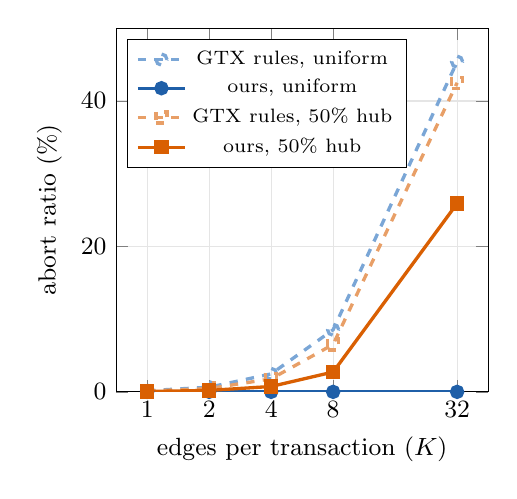
\begin{tikzpicture}
\begin{axis}[width=0.52\textwidth, height=6.2cm,
  xmode=log, log basis x=2, xtick={1,2,4,8,32}, xticklabels={1,2,4,8,32},
  ymin=0, ymax=50, grid=major, grid style={black!10},
  xlabel={edges per transaction ($K$)}, ylabel={abort ratio (\%)},
  tick label style={font=\small}, label style={font=\small},
  legend style={font=\scriptsize, at={(0.03,0.97)}, anchor=north west}]
\addplot[cCONS, very thick, dashed, mark=o] coordinates {(1,0.16)(2,0.64)(4,2.47)(8,8.54)(32,45.4)};
\addlegendentry{GTX rules, uniform}
\addplot[cGTX, very thick, mark=*] coordinates {(1,0)(2,0)(4,0)(8,0)(32,0)};
\addlegendentry{ours, uniform}
\addplot[cHUB!60, very thick, dashed, mark=square] coordinates {(1,0.11)(2,0.46)(4,1.79)(8,6.52)(32,42.5)};
\addlegendentry{GTX rules, 50\% hub}
\addplot[cHUB, very thick, mark=square*] coordinates {(1,0.05)(2,0.20)(4,0.74)(8,2.73)(32,25.9)};
\addlegendentry{ours, 50\% hub}
\end{axis}
\end{tikzpicture}\hfill
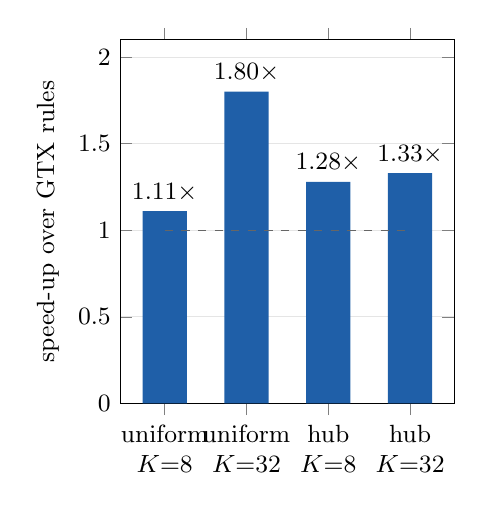
\begin{tikzpicture}
\begin{axis}[width=0.48\textwidth, height=6.2cm, ybar, bar width=16pt,
  ymin=0, ymax=2.1, symbolic x coords={u8,u32,h8,h32}, xtick=data,
  xticklabels={{uniform\\$K{=}8$},{uniform\\$K{=}32$},{hub\\$K{=}8$},{hub\\$K{=}32$}},
  xticklabel style={align=center, font=\small}, tick label style={font=\small},
  ylabel={speed-up over GTX rules}, label style={font=\small}, ymajorgrids, grid style={black!10},
  enlarge x limits=0.18, nodes near coords, nodes near coords style={font=\small},
  point meta=explicit symbolic]
\addplot[fill=cGTX, draw=none] coordinates {(u8,1.11)[$1.11\times$] (u32,1.80)[$1.80\times$] (h8,1.28)[$1.28\times$] (h32,1.33)[$1.33\times$]};
\draw[dashed, black!60] (axis cs:u8,1) -- (axis cs:h32,1);
\end{axis}
\end{tikzpicture}
\caption{Left: fraction of attempts that abort. With GTX's rule, aborts grow with transaction size to 45\%; with ours
they are zero on uniform graphs, and on the hub the remaining 26\% are true conflicts on the same edges. Right: the
resulting throughput gain.}
\label{fig:aborts}
\end{figure}

\textbf{How to read it:} an abort is wasted work. With GTX's rule, transactions that touch \emph{different} edges still
abort each other when those edges share a chain, and the bigger the transaction, the more likely that is. At 32 edges
per transaction almost half of all attempts are thrown away. Checking conflicts per edge removes all of those false
aborts, which makes the system $1.8\times$ faster at that size. At $K=1$ the two are within a few percent, as expected,
because false conflicts are rare for single-edge transactions.

\subsubsection*{Benchmark 3: realistic mixes and concurrent readers}
\begin{figure}[H]
\centering
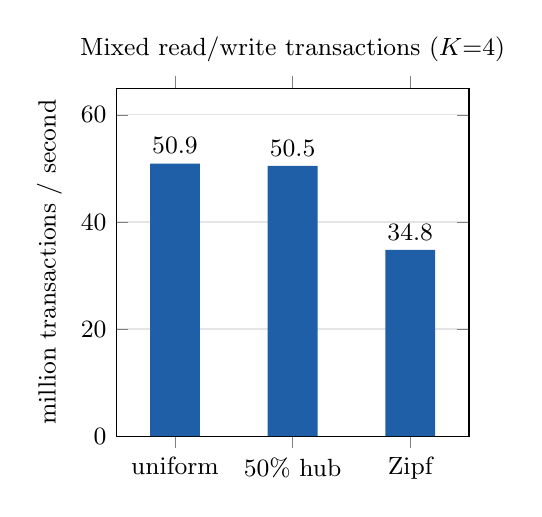
\begin{tikzpicture}
\begin{axis}[width=0.50\textwidth, height=6.0cm, ybar, bar width=18pt,
  ymin=0, ymax=65, symbolic x coords={U,H,Z}, xtick=data,
  xticklabels={uniform, 50\% hub, Zipf}, tick label style={font=\small},
  ylabel={million transactions / second}, label style={font=\small}, ymajorgrids, grid style={black!10},
  enlarge x limits=0.25, nodes near coords, nodes near coords style={font=\small},
  title={\small Mixed read/write transactions ($K{=}4$)}]
\addplot[fill=cGTX, draw=none] coordinates {(U,50.9) (H,50.5) (Z,34.8)};
\end{axis}
\end{tikzpicture}\hfill
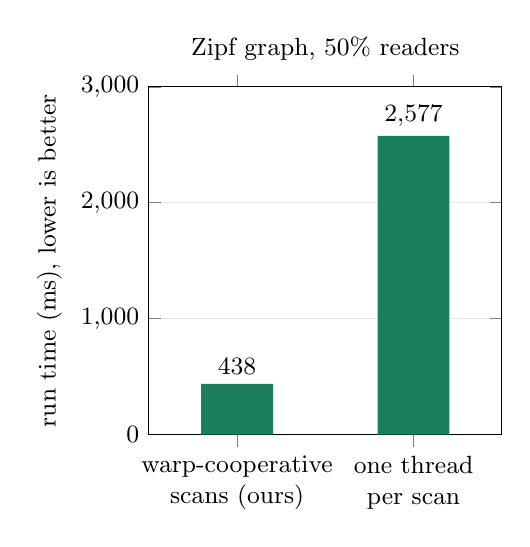
\begin{tikzpicture}
\begin{axis}[width=0.50\textwidth, height=6.0cm, ybar, bar width=26pt,
  ymin=0, ymax=3000, symbolic x coords={C,L}, xtick=data,
  xticklabels={{warp-cooperative\\scans (ours)},{one thread\\per scan}},
  xticklabel style={align=center, font=\small}, tick label style={font=\small},
  ylabel={run time (ms), lower is better}, label style={font=\small}, ymajorgrids, grid style={black!10},
  enlarge x limits=0.5, nodes near coords, nodes near coords style={font=\small},
  title={\small Zipf graph, 50\% readers}]
\addplot[fill=cGRN, draw=none] coordinates {(C,438) (L,2577)};
\end{axis}
\end{tikzpicture}
\caption{Left: committed transactions per second for a mix of 40\% inserts, 30\% deletes and 30\% reads. Right: letting
all 32 threads of a warp scan one vertex together is $5.9\times$ faster than one thread per scan.}
\label{fig:mix}
\end{figure}

\begin{center}
\begin{tabular}{@{}lrrr@{}}
\toprule
Mixed workload ($K=4$) & transactions/s & effective edges/s & abort ratio \\
\midrule
Uniform & 50.9 M & 140 M & 1.1\% \\
50\% hub & 50.5 M & 105 M & 1.9\% \\
Zipf & 34.8 M & 94 M & 1.1\% \\
\bottomrule
\end{tabular}
\end{center}

\textbf{Readers.} On an R-MAT graph where \textbf{90\%} of transactions are read-only (10\% of their operations scan a
whole vertex's neighbour list):
\begin{itemize}
\item \textbf{17.3 million} transactions per second;
\item overall abort ratio \textbf{0.03\%};
\item read-only transactions: half finish within \textbf{0.64~ms} (p50), 99\% within \textbf{2.4~ms} (p99), including
  scans. Readers never wait and never abort.
\end{itemize}

\textbf{Other supporting numbers} (use if asked): delete/insert churn with single-edge transactions runs at 156 million
effective edges/s (uniform) and 144 million/s (R-MAT); the batch-commit machinery costs only 9.6--15.5\% of the GPU's
time for single-edge inserts.

\begin{sayit}
``How do readers stay consistent? Transactions commit in numbered batches. A whole warp joins a batch with a single
atomic operation. One special thread closes each batch and, only when every writer in it is done, announces it as
complete by moving a number we call the frontier. A reader just reads the frontier and ignores anything newer
[Figure~\ref{fig:epochs}]. So a reader sees all of a transaction or none of it, and never waits. Our first design
retried when the batch number changed, and since it changes every microsecond, it could spin for seconds; making it one
atomic operation fixed that.

How do we know it's correct? GPU concurrency bugs don't crash; they give a wrong answer once in a million. So we record
every operation's result and a checker replays the whole history and verifies every single read. All 48 adversarial
scenarios pass. We also broke the system on purpose three ways; the checker caught all three, and two of them would
have passed the usual `compare the final graph' test.

First numbers, on a laptop RTX 4060 with a million-vertex graph: 140 to 180 million edge inserts per second, steady as
transactions grow [Figure~\ref{fig:ksweep}]. Our per-edge conflict rule removes the unnecessary aborts of GTX's rule:
at 32 edges per transaction GTX's rule throws away 45\% of attempts, ours none, which makes us 1.8 times faster
[Figure~\ref{fig:aborts}]. With 90\% readers we run 17 million transactions per second and 99\% of reads finish within
2.4 milliseconds.

Next stage: a stricter correctness mode, the full comparison against other GPU systems, and cleaning up old versions.
Thank you, questions?''
\end{sayit}

\begin{askme}
\textbf{How does it compare to other systems?} That is the next stage: the competing approaches (locking and GPU
transactional memory) are implemented and the full comparison is the next milestone.

\textbf{Why is the hub workload slower at $K=32$?} 32-edge transactions that all touch the same vertex genuinely
conflict; those 26\% aborts are real conflicts, not false ones. GTX's rule adds 17 more percentage points of false ones.

\textbf{Why is ``effective edges/s'' lower than transactions/s on the hub?} Many hub inserts try to add an edge that
already exists; that is a no-op and is not counted as an effective change.

\textbf{Why a laptop GPU?} It is the hardware we have. All systems in the full comparison run on the same machine,
so comparisons are fair; absolute numbers would be higher on a data-centre GPU.

\textbf{What is the advancer? Isn't one thread a bottleneck?} It only moves a counter forward; commit machinery is
9.6--15.5\% of GPU time in the worst (single-edge) case.
\end{askme}

\begin{slides}
\begin{enumerate}[leftmargin=*]
\item ``Readers see complete batches'': Figure~\ref{fig:epochs}, plus the livelock story in one sentence.
\item ``We check every read'': the list of checks and the results (48/48, 3/3 bugs caught).
\item ``Speed as transactions grow'': Figure~\ref{fig:ksweep}.
\item ``Fewer wasted attempts'': Figure~\ref{fig:aborts}.
\item ``Readers never wait'': the reader numbers and Figure~\ref{fig:mix} (right).
\item ``Next stage'' and questions.
\end{enumerate}
\end{slides}

\newpage
%% ==========================================================================================
\section{What we are \emph{not} presenting today}
\label{sec:later}

\begin{dont}
These exist and are done, but they are the second half of the project. Do not bring them up; if asked, say
``that is our next milestone''.
\begin{itemize}
\item \textbf{Comparison against other systems} (two-phase locking, TL2 GPU transactional memory, non-transactional
  updates, GPMA+) and the large speedups from it.
\item \textbf{Serializable mode} (the stricter correctness level) and the write-skew test.
\item \textbf{Hypothesis tests / ablations}, including the finding that one-atomic-per-warp reservation helps only a
  little (3--11\%).
\item \textbf{Where we are slower} (uncontended small transactions versus locking) and the \textbf{memory overhead}
  (2.5--20$\times$), which cleanup of old versions will address.
\item The list of protocol bugs found and fixed (except the livelock story above), memory-ordering details and formal
  invariants.
\end{itemize}
\end{dont}

%% ==========================================================================================
\section{Team preparation checklist}
\begin{itemize}
\item Everyone: read Sections~\ref{sec:glossary} and \ref{sec:big}, your own section, and the other two ``one sentence''
  boxes.
\item Presenter 1: be able to explain the torn-read example and why GPU transactional memory struggles with hub vertices.
\item Presenter 2: be able to walk Figure~\ref{fig:chain} (which version a reader sees) and Figure~\ref{fig:cas}
  (who wins a race) without notes.
\item Presenter 3: be able to explain why a reader can never see half a transaction (Figure~\ref{fig:epochs}) and how
  to read Figures~\ref{fig:ksweep} and \ref{fig:aborts}.
\item Rehearse the two handoff sentences so the talk flows as one story.
\end{itemize}

\textbf{Where the numbers come from} (in case someone asks to see the data): \code{results/summary.csv},
\code{results/speedups.csv}, \code{results/correctness\_suite.txt} and \code{results/mutation\_final\_state.txt} in the
project repository; the full technical report is \code{paper/GTX-GPU\_Technical\_Report.pdf}.

\end{document}
